\documentclass[12pt, titlepage]{article}

\usepackage{fullpage}
\usepackage[round]{natbib}
\usepackage{multirow}
\usepackage{booktabs}
\usepackage{tabularx}
\usepackage{graphicx}
\usepackage{float}
\usepackage{hyperref}
\usepackage[normalem]{ulem}
\usepackage{xcolor}
\hypersetup{
    colorlinks,
    citecolor=black,
    filecolor=black,
    linkcolor=red,
    urlcolor=blue
}
\usepackage[round]{natbib}

\newcounter{acnum}
\newcommand{\actheacnum}{AC\theacnum}
\newcommand{\acref}[1]{AC\ref{#1}}

\newcounter{ucnum}
\newcommand{\uctheucnum}{UC\theucnum}
\newcommand{\uref}[1]{UC\ref{#1}}

\newcounter{mnum}
\newcommand{\mthemnum}{M\themnum}
\newcommand{\mref}[1]{M\ref{#1}}

\title{SE 3XA3: Software Requirements Specification\\Title of Project}

\author{Team \#204, Trident Inc.
		\\ Harshil Modi, modih1
		\\ Justin Prez, prezj
		\\ Justin Rosner, rosnej1
}

\date{\today}


\begin{document}

\maketitle

\pagenumbering{roman}
\tableofcontents
\listoftables
\listoffigures

\begin{table}[H]
\caption{Revision History} \label{TblRevisionHistory}
\begin{tabularx}{\textwidth}{llX}
\toprule
\textbf{Date} & \textbf{Developer(s)} & \textbf{Change}\\
\midrule
2020-03-09 & Justin Rosner, Justin Prez, Harshil Modi & Initial write-up of MG document\\

\textcolor{red}{2020-04-05} & \textcolor{red}{Justin Rosner, Justin Prez, Harshil Modi} & \textcolor{red}{Revision 1 of MG document}\\
\bottomrule
\end{tabularx}
\end{table}

\newpage

\pagenumbering{arabic}

\section{Introduction}
\subsection{Overview}
Mastermind is a famous 1970's Mordecai Meirowitz game implemented as an android application \sout{implemented} using Dart and Flutter. The goal of our project is the bring Mastermind back as the game that can be enjoyed by people of all ages. By developing an app version of the game, people will be able to play the game in their free time, or on-the-go. The Mastermind development team have added numerous requirements that the open source version failed to address, as seen in the \href{https://gitlab.cas.mcmaster.ca/rosnej1/open-mastermind/-/blob/master/Doc/SRS/SRS.pdf}{SRS}. \textcolor{red}{The MG aims to separate these requirements into modules of similar functionality.} The primary focus of the team is code modularization, maintainability, interoperability, and robustness. For a breakdown of the modules the team has deemed important, see the \href{https://gitlab.cas.mcmaster.ca/rosnej1/open-mastermind/-/tree/master/Doc/Design/MIS/MIS.pdf}{Module Interface Specification}. 

\subsection{Scope}
The scope of the project is to create a more interactive implementation of the Mastermind game. As the rules of the game of Mastermind are fairly straightforward, the development team will have no issues recreating the game in its entirety. The app will be developed with Dart/Flutter, allowing for deployment on both iOS and Android platforms through the Apple Store and Google Play Store.

\subsection{Module Guide Purpose}
When developing a mobile game, there are numerous components that fit together to form the final product. The purpose of the Module Guide is to provide an overview of how the team decided to decompose the components of Mastermind and provide an explanation on how the components interact with each other. Furthermore, the module guide will be used by the design team to ensure the consistency between the implementation and specification entitled through the documentation. Finally, the Module guide will provide developers with a way of understanding the implementation structure of Mastermind. 

% \subsection{Introduction part 2}

% Decomposing a system into modules is a commonly accepted approach to developing
% software.  A module is a work assignment for a programmer or programming.  We advocate a decomposition
% based on the principle of information hiding,   code  modularization,  maintainability, and  interoperability. This
% principle supports design for change, because the ``secrets'' that each module
% hides represent likely future changes.  Design for change is valuable in SC,
% where modifications are frequent, especially during initial development as the
% solution space is explored.  

% Our design follows the rules layed out by the MIS, as follows:
% \begin{itemize}
% \item System details that are likely to change independently should be the
%   secrets of separate modules.
% \item Each data structure is used in only one module.
% \item Any other program that requires information stored in a module's data
%   structures must obtain it by calling access programs belonging to that module.
% \end{itemize}

% After completing the first stage of the design, the Software Requirements
% Specification (SRS), the Module Guide (MG) is developed. The MG
% specifies the modular structure of the system and is intended to allow both
% designers and maintainers to easily identify the parts of the software.  The
% potential readers of this document are as follows:

% \begin{itemize}
% \item New project members: This document can be a guide for a new project member
%   to easily understand the overall structure and quickly find the
%   relevant modules they are searching for.
% \item Maintainers: The hierarchical structure of the module guide improves the
%   maintainers' understanding when they need to make changes to the system. It is
%   important for a maintainer to update the relevant sections of the document
%   after changes have been made.
% \item Designers: Once the module guide has been written, it can be used to
%   check for consistency, feasibility and flexibility. Designers can verify the
%   system in various ways, such as consistency among modules, feasibility of the
%   decomposition, and flexibility of the design.
% \end{itemize}

% The rest of the document is organized as follows. Section
% \ref{SecChange} lists the anticipated and unlikely changes of the software
% requirements. Section \ref{SecMH} summarizes the module decomposition that
% was constructed according to the likely changes. Section \ref{SecConnection}
% specifies the connections between the software requirements and the
% modules. Section \ref{SecMD} gives a detailed description of the
% modules. Section \ref{SecTM} includes two traceability matrices. One checks
% the completeness of the design against the requirements provided in the SRS. The
% other shows the relation between anticipated changes and the modules. Section
% \ref{SecUse} describes the use relation between modules.

\section{Anticipated and Unlikely Changes} \label{SecChange}
This section of the Module Guide outlines possible changes to the design that the development team has considered but not yet implemented. These changes are broken down into two categories; Anticipated changes (\ref{SecAchange}) that the development team will start to work on in the near future, and Unlikely Changes (\ref{SecUchange}) that are more theory based and not realistic for the development team.

\subsection{Anticipated Changes} \label{SecAchange}

\begin{description}
\item[\refstepcounter{acnum} \actheacnum \label{ac1}:] The specific
  hardware on which the software is running (i.e. a new phone or tablet is released).
\item[\refstepcounter{acnum} \actheacnum \label{ac2}:] The operating system that the software runs on.
\item[\refstepcounter{acnum} \actheacnum \label{ac3}:] The format and layout of the game board.
\item[\refstepcounter{acnum} \actheacnum \label{ac4}:] The format and layout of the game menus.
\item[\refstepcounter{acnum} \actheacnum \label{ac5}:] The appearance of the buttons.
\end{description}

\subsection{Unlikely Changes} \label{SecUchange}

% The module design should be as general as possible. However, a general system is
% more complex. Sometimes this complexity is not necessary. Fixing some design
% decisions at the system architecture stage can simplify the software design. If
% these decision should later need to be changed, then many parts of the design
% will potentially need to be modified. Hence, it is not intended that these
% decisions will be changed.

\begin{description}
\item[\refstepcounter{ucnum} \uctheucnum \label{ucIO}:] Input devices. Given the rise of virtual and augmented reality in the last couple of years, it is possible that the team may wish to make this the focus of the user's interactions with Mastermind. Given the scope and the time required to make this change, it is unlikely that the development team will choose to replace the touch screen based interaction system currently in place.
\item[\refstepcounter{ucnum} \uctheucnum \label{ucChangeRules}:] Changes to the rules of the game. Changing the rules of the game would cause for changes to occur in the game board module, menu module, and both the game logic controller and the game state controller. Due to changes occurring in more than one module, it becomes a very unlikely change for the development team to make.
\end{description}

\section{Module Hierarchy} \label{SecMH}

This section provides an overview of the module design. Modules are summarized
in a hierarchy decomposed by secrets in Table \ref{TblMH}. The modules listed
below, which are leaves in the hierarchy tree, are the modules that will
actually be implemented.

\begin{description}
\item [\refstepcounter{mnum} \mthemnum \label{m1}:] Android Emulator
\item [\refstepcounter{mnum} \mthemnum \label{m2}:] Game Board Module
\item [\refstepcounter{mnum} \mthemnum \label{m3}:] Menu Module
\item [\refstepcounter{mnum} \mthemnum \label{m4}:] Button Module
\item [\refstepcounter{mnum} \mthemnum \label{m5}:] Game Board Controller
\item [\refstepcounter{mnum} \mthemnum \label{m6}:] Types Module

\end{description}


\begin{table}[H]
\centering
\begin{tabular}{p{0.3\textwidth} p{0.6\textwidth}}
\toprule
\textbf{Level 1} & \textbf{Level 2}\\
\midrule

{Hardware-Hiding Module} & Android Emulator \\
\midrule

\multirow{3}{0.3\textwidth}{Behaviour-Hiding Module} & Game Board Module\\
& Menu Module \\
& Button Module \\
& Types Module \\
\midrule

{Software Decision Module} & Game Board Controller\\
\bottomrule

\end{tabular}
\caption{Module Hierarchy}
\label{TblMH}
\end{table}

\section{Connection Between Requirements and Design} \label{SecConnection}

This application was designed to satisfy all the requirements outlined in
the \href{https://gitlab.cas.mcmaster.ca/rosnej1/open-mastermind/-/blob/master/Doc/SRS/SRS.pdf}{SRS Document}. In this stage, Mastermind is decomposed into modules to fulfill the functional requirements, such as displaying the game board on an Android/iOS device. The connection between requirements and modules is listed in Table \ref{TblRT}.

\section{Module Decomposition} \label{SecMD}

Module decomposition is critical for improving the principle of ``information hiding''. Information hiding significantly reduces the complexity, while improving the maintainability and scalability of the program. Each module below contains fields for \emph{Secrets}, \emph{Services} and \emph{Implemented By}.   The \emph{Secrets} field describes the design decisions hidden by the module. The \emph{Services} field details what the module will do not documenting how to do it. The \emph{Implemented By} field suggests the implementing software. 


\subsection{Hardware Hiding Module: Android Emulator (\mref{m1})}

\begin{description}
\item[Secrets:] The data structures and algorithms used to implement the virtual
  android emulator, track and manipulate the windows displayed to the screen.
\item[Services:] Serves as virtual hardware to emulate an android smartphone, able to run applications, accept user input and display output to the screen.
\item[Implemented By:]  \emph{OS}
\end{description}

\subsection{Behaviour-Hiding Module}

\begin{description}
\item[Secrets:]The contents of the required behaviours for the Game Board, Menu, Button and Types Modules.
\item[Services:]The programs included affect the visible appearance of the game as described in the software requirements specification (SRS)
  documents. These modules serve as a communication layer between the
  hardware-hiding module and the software decision module.
\item[Implemented By:] Mastermind
\end{description}

\subsubsection{Game Board Module (\mref{m2})}

\begin{description}
\item[Secrets:]The functions and state variables used to create an instance of the game board and draw it to the screen.
\item[Services:] Draws the game board to the screen, and updates the visible game board based on user input.
\item[Implemented By:] Mastermind
\end{description}

\subsubsection{Menu Module (\mref{m3})}

\begin{description}
\item[Secrets:] The functions and state variables used to create the menu screen.
\item[Services:] Accepts user input for selections on the menu screen.
\item[Implemented By:] Mastermind
\end{description}

\subsubsection{Button Module (\mref{m4})}

\begin{description}
\item[Secrets:] The functions and state variables used draw the button to the screen.
\item[Services:] Draws the buttons of different colours to the screen.
\item[Implemented By:]  \emph{OS}
\end{description}

\subsubsection{Types Module (\mref{m6})}

\begin{description}
\item[Secrets:] \sout{N/A.} \textcolor{red}{The implementation of various types needed for the rest of the modules.}
\item[Services:] The exported types from this module are to be used in other modules. 
\item[Implemented By:]  Mastermind
\end{description}

\subsection{Software Decision Module}

\begin{description}
\item[Secrets:] Algorithms and data structures used for implementing the game rules and tracking the state of the Game Board.
\item[Services:] Includes data structure and algorithms used in to implement the game that the user does not directly interact with. 
  % Changes in these modules are more likely to be motivated by a desire to
  % improve performance than by externally imposed changes.
\item[Implemented By:] --
\end{description}

\subsubsection{Game Board Controller (\mref{m5})}

\begin{description}
\item[Secrets:] Algorithm used to implement the rules of the game and logic of the game board.
\item[Services:] Includes algorithms that are used for interpreting user input, displaying correct output, and checking for win/lose conditions.
\item[Implemented By:] Mastermind
\end{description}

\section{Traceability Matrix} \label{SecTM}

This section shows two traceability matrices: between the modules and the
requirements and between the modules and the anticipated changes.

% the table should use mref, the requirements should be named, use something
% like fref
\begin{table}[H]
\centering
\begin{tabular}{p{0.2\textwidth} p{0.6\textwidth}}
\toprule
\textbf{Req.} & \textbf{Modules}\\
\midrule
REQ1 & \mref{m1}\\
REQ2 & \mref{m2}, \mref{m4}\\
REQ3 & \mref{m2}, \mref{m4}\\
REQ4 & \mref{m2}, \mref{m4}\\
REQ5 & \mref{m2}, \mref{m4}\\
REQ6 & \mref{m2}, \mref{m4}\\
REQ7 & \mref{m2}, \mref{m4}\\
REQ8 & \mref{m2}, \mref{m5}, \mref{m1}\\
REQ9 & \mref{m3}, \mref{m1}\\
REQ10 & \mref{m5}, \mref{m1}\\
\textcolor{red}{REQ11} & \textcolor{red}{\mref{m2}, \mref{m5}}\\
\textcolor{red}{REQ12} & \textcolor{red}{\mref{m2}, \mref{m5}}\\
\textcolor{red}{REQ13} & \textcolor{red}{\mref{m2}, \mref{m5}}\\
\textcolor{red}{REQ14} & \textcolor{red}{\mref{m2}, \mref{m5}}\\
\bottomrule
\end{tabular}
\caption{Trace Between Requirements and Modules}
\label{TblRT}
\end{table}

\begin{table}[H]
\centering
\begin{tabular}{p{0.2\textwidth} p{0.6\textwidth}}
\toprule
\textbf{AC} & \textbf{Modules}\\
\midrule
\acref{ac1} & \mref{m1}\\
\acref{ac2} & \mref{m1}\\
\acref{ac3} & \mref{m2}\\
\acref{ac4} & \mref{m3}\\
\acref{ac5} & \mref{m4}\\
\bottomrule
\end{tabular}
\caption{Trace Between Anticipated Changes and Modules}
\label{TblACT}
\end{table}

\section{Use Hierarchy Between Modules} \label{SecUse}

In this section, the uses hierarchy between the interacting modules is
provided. It can be seen that the hierarchy represented below is an example of a directed acyclic graph
(DAG). Meaning that if the Game Board Controller is dependent on the Game Board Module (and on a higher level in the hierarchy), then the Game Board Module cannot be dependent on the Game Board Controller. Modules in the higher level of the hierarchy have simpler implementations
because they use 'secrets' from the lower levels.

\begin{figure}[H]
\centering
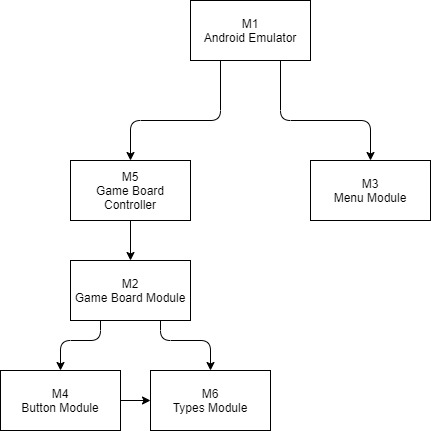
\includegraphics[width=0.7\textwidth]{module_hierarchy.jpg}
\caption{Use hierarchy among modules}
\label{FigUH}
\end{figure}

%\section*{References}

\bibliographystyle {plainnat}
\bibliography {MG}

\end{document}

